\chapter[Lecture 14]{}\label{lec14}

\begin{minipage}[c]{6.5cm}
\begin{figure}[H]
\centering
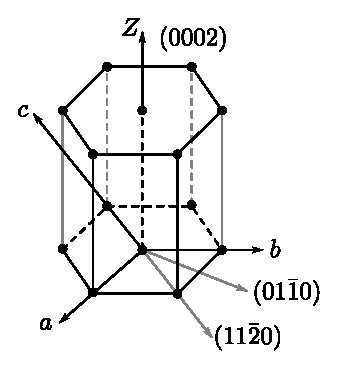
\includegraphics{images/lecture14/fig1.eps}
\end{figure}
\end{minipage}
\qquad
\begin{minipage}[c]{6.5cm}
\begin{figure}[H]
\centering
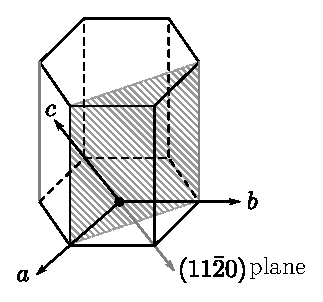
\includegraphics{images/lecture14/fig2.eps}
\end{figure}
\end{minipage}

\section*{HCP lattice}
$a=b\neq c$\quad $\alpha=\beta=90^{\circ}$\quad $\gamma=120^{\circ}$
\begin{align*}
b_{1} &= \dfrac{\sqrt{3}}{2}a\widehat{x}-\dfrac{a}{2}\widehat{y}\\
b_{2} &= a\widehat{y}\quad b_{3}=c\widehat{z}
\end{align*}

\section*{Structure determination}

Interatomic distance $\sim A^{0}=10^{-8}$cm.; $10^{-10}$ meter.

To probe such length scale, the wavelength of the probe has to be of same order or smaller.

$\therefore$ Energy $=hw=\dfrac{hc}{\lambda}=\dfrac{hc}{10^{-8}}$cm $\approx 12.3\times 10^{3}$ eV.

\medskip
\noindent
{\bf Bragg formulation :} W.H Bragg and W.L. Bragg (1913)

Bragg found that characteristic pattern of reflected $x$-radiation is significantly different for solid (crystalline) compared to liquid.

They proposed that all crystals are made of parallel plane of ions spaced by a distance `$d$'.

Assumptions
\begin{itemize}
\item[(i)] Reflection is specular.

\item[(ii)] Reflected rays from successive planes interface constructively.
\end{itemize}
\begin{figure}[H]
\centering
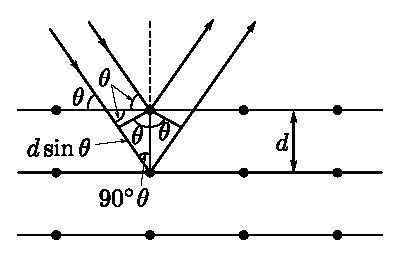
\includegraphics{images/lecture14/fig3.eps}
\end{figure}

Path difference
$$
\fbox{
$\begin{array}{l}
= 2d \sin\theta\\
= n\lambda
\end{array}
$
}
$$
for constructor interference.

$n\to$ integer

= order of reflection.

\section*{Von Lane formulation}

No particular lattice plane is singled out.

No ad $h_{c}$ assumption of specular reflection.
\begin{itemize}
\item Lattice consists of identical microscopic objects and radiate in all directions.
\begin{figure}[H]
\centering
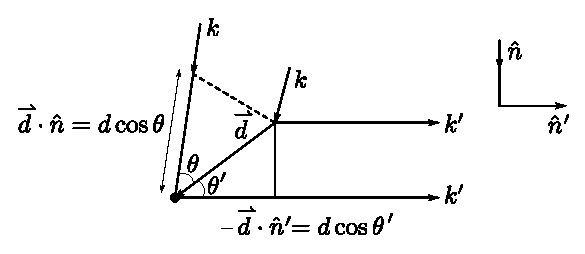
\includegraphics{images/lecture14/fig4.eps}
\end{figure}

\item Lets assume $\widehat{n}\to$ incident direction.

$\widehat{n}'\to$ scattered direction.

$k=\dfrac{2\pi\widehat{n}}{\lambda}$\quad $k'=\dfrac{2\pi\widehat{n}'}{\lambda}$

Path difference $=d\cos\theta+d\cos \theta'=\overrightarrow{d}(\widehat{n}-\widehat{n}')=m\lambda$ (integer) for constructive interference.
$$
\therefore\quad \fbox{$\overrightarrow{d}(\overrightarrow{k}-\overrightarrow{k}')=2\pi m$}
$$
For an array of Bravais lattice vectors.
$$
\fbox{$\overrightarrow{R}(\overrightarrow{k}-\overrightarrow{k}')=2\pi m$}\quad \therefore \ \fbox{$e^{i(\overrightarrow{k}'-\overrightarrow{k})\cdot R}=1$}
$$
looks quite similar to the definition used for reciprocal lattice.
$$
e^{ik\cdot R}=1
$$
$\therefore$ The Reciprocal Lattice vector \fbox{$\overrightarrow{k}=\overrightarrow{k}'-\overrightarrow{k}$} (Lane condition) leads to constructive interference.
\end{itemize}

\section*{Alternative definitions}

If $(k'-k)$ is a Bravais lattice vector, $(\overrightarrow{k}-\overrightarrow{k}')$ will also be a Bravais lattice vector.

Assuming $\overrightarrow{k}=\overrightarrow{k}-\overrightarrow{k}'$, $\overrightarrow{k}$ and $\overrightarrow{k}'$ have same magnitude 
\begin{align*}
\therefore\quad & |k'|=|\overrightarrow{k}-\overrightarrow{K}|=|k|\\
\therefore\quad & k^{2}=k^{2}+k^{2}-2\overrightarrow{k}\cdot \overrightarrow{k}\quad \text{or}\quad \fbox{$\widehat{k}\cdot \widehat{K}=\dfrac{1}{2}|k|$}
\end{align*}
$\Rightarrow$ Component of incident wave vector, $k$ along $\widehat{k}$ must be half the length of $K$.

Incident vector $\overrightarrow{k}$ will satisfy Lane condition if and only if the tip of $\overrightarrow{k}$ lies on a plane perpendicular bisector of the reciprocal lattice vector.

The plane is called Bragg plane.
\begin{figure}[H]
\centering
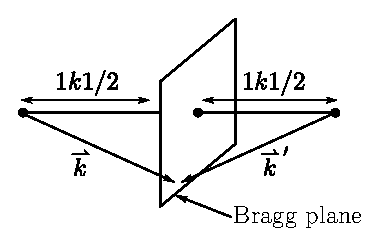
\includegraphics{images/lecture14/fig5.eps}
\end{figure}

\section*{Equivalence of Bragg and Lane formulation}

Lane condition $\overrightarrow{K}=\overrightarrow{k}'-\overrightarrow{k}$

Since the scattering is elastic scattering $|k|=|k'|$.

$\therefore$ Scattering can be viewed as Bragg reflection with Bragg angle $\theta$ from the family of direct lattice planes perpendicular to $\overrightarrow{K}$.

Lane condition involves reciprocal lattice Bragg condition $\to$ real lattice.

If $d$ is distance between planes, the shortest reciprocal lattice vector parallel to $\overrightarrow{K}$ is $\overrightarrow{K}_{0}=\dfrac{2\pi}{d}$
\begin{figure}[H]
\centering
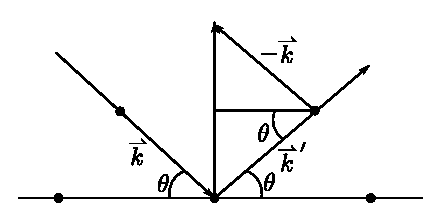
\includegraphics{images/lecture14/fig6.eps}
\end{figure}

$\therefore \ K=\dfrac{2\pi n}{d}$

$|K|=2|k|\sin \theta$

$\therefore \ 2k\sin \theta=\dfrac{2\pi n}{d}$\quad $k=\dfrac{2\pi}{\lambda}$
$$
a\fbox{$2d\sin\theta=\dfrac{2\pi n}{k}=n\lambda$}
$$
\begin{itemize}
\item Since reciprocal lattice is visualized much better than real lattice, Lane condition is simpler to work with than the Bragg condition.
\end{itemize}

\section*{Ewald Construction (P.P. Ewald (1913))}

Lane condition $\Delta k=G$ can be expressed in another way to get Lane equations. Take scalar product of both $\Delta k$ and $G$ with $\overrightarrow{a}_{1}$, $\overrightarrow{a}_{2}$ and $\overrightarrow{a}_{3}$
\begin{gather*}
G=v_{1}b_{1}+v_{2}b_{2}+v_{3}b_{3}\\
\fbox{$\overrightarrow{a}_{1}\cdot \Delta k=2\pi v_{1}$}\quad \fbox{$a_{2}\cdot \Delta k=2\pi v_{2}$}\quad \fbox{$a_{3}\cdot \Delta k=2\pi v_{3}$}
\end{gather*}
\begin{quote}
$a_{1}\cdot \Delta k=2\pi v_{1}$ suggests that $\Delta k$ lies on a certain Cone about $a_{1}$

$a_{2}\cdot \Delta k=2\pi v_{2}$ suggests, $\Delta k$ lies on a Cone about $a_{2}$

$a_{3}\cdot \Delta k=2\pi v_{3}$ suggest $\Delta k$ lies on a Cone about $a_{3}$
\end{quote}
Satisfaction of all these three conditions together is a Herculean task $\to$ may happen accidentally.

To find an easy way P.P. Ewald made a beautiful construction.
\begin{figure}[H]
\centering
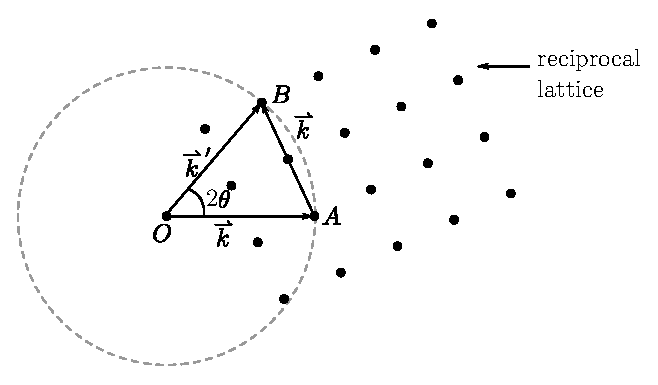
\includegraphics{images/lecture14/fig7.eps}
\end{figure}
\begin{itemize}
\item[$\to$] Draw the incident wave vector, $\overrightarrow{k}$ in such a way it terminates on a reciprocal lattice point.

\item[$\to$] Draw a sphere of radius $k\left(=\dfrac{2\pi}{\lambda}\right)$ with origin at the initial point of $\overrightarrow{k}$.

\item[$\to$] A diffracted beam will be formed if the sphere intersects any other reciprocal lattice point, say $B$ in the figure. 

\item[$\to$] $\overrightarrow{OB}$ is $\overrightarrow{k}'$ makes an angle $\angle{BOA}$ with $\overrightarrow{k}=2\theta$

\item[$\to$] $\overrightarrow{AB}=\overrightarrow{k}$ is a reciprocal lattice vector, so Lane condition satisfies.

\fbox{$\overrightarrow{k}'=\overrightarrow{k}+\overrightarrow{k}$}\quad $\theta=$ Bragg angle.
\end{itemize}

\section*{Definition of Brillouin Zone}

We found
\begin{align*}
&\fbox{$\overrightarrow{k}\cdot \widehat{k}=\dfrac{1}{2}|\overrightarrow{k}|$}\tag{A}\label{lec14-eqA}\\
\text{or}\quad & \overrightarrow{k}\cdot \dfrac{\overrightarrow{k}}{2}=\left(\dfrac{k}{2}\right)^{2}
\end{align*}
\begin{itemize}
\item[$\to$] Take a reciprocal lattice vector $\overrightarrow{K}$ from origin $(000)$ called $\Gamma$-point.

\item[$\to$] Construct a plane bisecting $\overrightarrow{K}$, this plane forms a zone boundary.

\item[$\to$] An $n$-ray beam will be diffracted if the wave vector $\overrightarrow{k}$ has the magnitude satisfied by equation \eqref{lec14-eqA}.

\item[$\to$] The diffracted beam will be in the direction of $\overrightarrow{k}-\overrightarrow{K}\Rightarrow \Delta \overrightarrow{k}=-\overrightarrow{K}$

[Remember Ewald construction, tip of $\overrightarrow{k}$ lands at reciprocal lattice point, which is opposite of $\overrightarrow{k}$ defined here. Then, $\overrightarrow{k}-\overrightarrow{k}$ comes]

\item[$\to$] Brillouin Construction exhibits all the wave vectors $\overrightarrow{k}$ which can be Bragg reflected by the crystal.
\begin{figure}[H]
\centering
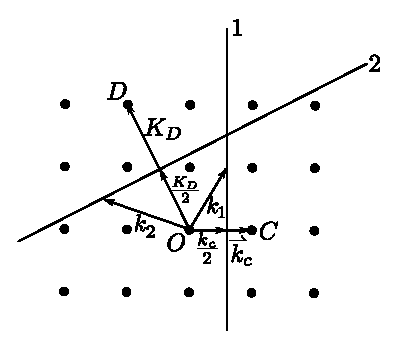
\includegraphics{images/lecture14/fig8.eps}
\end{figure}

\item[$\to$] Draw all possible planes in this way. The smallest volume enclosed in first Brillouin Zone.

\item[$\to$] Wigner Seitz cell of reciprocal lattice.
\end{itemize}

%page 3
\section*{Structure determination}
\begin{itemize}
\item[(i)] Lane Method : Keep the crystal fixed and incident $x$-ray direction fixed.
\begin{itemize}
\item[$\to$] Possibility of getting a reciprocal lattice point of Ewald sphere is less.

Use non monochromatic light $\lambda_{1}\leq \lambda \leq \lambda_{0}$

\item[$\to$] $\therefore$ The reciprocal points within the volume between the two spheres of radius $\dfrac{2\pi}{\lambda_{1}}$ and $\dfrac{2\pi}{\lambda_{0}}$ will contribute if they fall on any of the spheres.

\item[$\to$] Choose $\Delta \lambda=\lambda_{1}-\lambda_{0}$ optimum to have large no. of spots but not too large that makes the problem complex.

\item[$\to$] If $\overrightarrow{k}$ is aligned along a symmetry axis of the crystal, the pattern of spots will reflect the same symmetry.

\item[$\to$] Normally this method is used to orient a crystal in certain direction.
\end{itemize}

\item[(ii)] {\bf Rotating Crystal Method :}
\begin{itemize}
\item[$\to$] Keep $\overrightarrow{k}$ fixed ($\lambda=$ count and direction is fixed)

\item[$\to$] Rotate the crystal $\to$ reciprocal lattice will rotate.
\end{itemize}
Whenever a reciprocal lattice point falls on Ewald sphere (fixed in this case), a diffraction spot will appear.

Usually used for {\bf electron diffraction}, $\lambda$ can be make smaller than the lattice constant `$a$' simply by increasing electron energy $\to$ Ewald sphere is big. So one can get all possible points on detector to get the complete picture of the structure.

\item[(iii)] {\bf Power Diffraction (XRD) or Debye-Scherrer Method :}

This is similar to rotating crystal method.
\begin{itemize}
\item[$\to$] Make fine powder of the sample, so that they are isotropic giving all possible orientations for different grains.

\item[$\to$] Now find the diffraction peaks as a function of scattering angle.

\item[$\to$] Whenever Bragg condition is satisfied, a peak will appear.

\item[$\to$] Good for all kinds of sample (poly crystals, powder of simple crystals)
\end{itemize}
\end{itemize}

\section*{Diffraction by a crystal with a basis : Structure factor}

Lets assume incident and outgoing wave vector are $\overrightarrow{k}$ and $\overrightarrow{k}$ for an incident $x$-ray beam on a sample.
\begin{figure}[H]
\centering
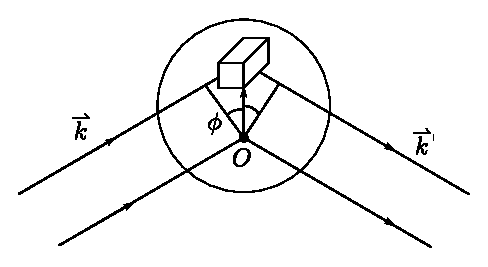
\includegraphics{images/lecture14/fig9.eps}
\end{figure}

Amplitude of scattered wave will depend on the local electron density, $n(r)$ at $\overrightarrow{r}$.

Total intensity of the scattered wave will be integral of $n(r)dV$ times the phase factor $e^{i(k-k')\cdot r}$.

In other words, the amplitude of the electric or magnetic field vectors in the scattered electromagnetic wave can be written as Scattering amplitude,
\begin{align*}
& F=\int dV \ n(r)\exp [i(\overrightarrow{k}-\overrightarrow{k'})\cdot r]\\
& a, \fbox{$F=ing dV \ n(r) \exp [-i\Delta k\cdot r]$}k-k'=-\Delta k\tag{1}\label{lec14-eq1}
\end{align*}
$\Delta k$ is the measure of change in wave vector and called scattering vector.

One can express $n(r)$ in Fourier expansion as discussed before.
\begin{equation*}
\therefore\quad \fbox{$F=\sum\limits_{G}\int dV \ n_{G}\exp [i(G-\Delta k)\cdot r]$}\tag{2}\label{lec14-eq2}
\end{equation*}
If \fbox{$\Delta k=G$},  $F=Vn_{G}$ and for $sk\neq G$, $F$ is negligibly small diffraction condition.

In Eqn. \eqref{lec14-eq1}, if we substitute $\Delta k=G$, we get
$$
\fbox{$F_{G}=N\int\limits_{\text{cell}}dV \ n(r)e^{-iG.r}=NS_{G}$}
$$
$S_{G}$ is called the structure factor. The integral is over one cell and the origin at one corner of the cell.

If all the atoms in the cell are not identical, it has a basis, scattering factor will depend on the contribution from all the atoms within the basis.

Now, if $n_{j}$ is electron concentration function of atom `$j$' located at $r_{j}$, one can write $n(r)$ as sum of the contribution coming from all the atoms in the basis
\begin{align*}
\therefore\quad n(r) &= \sum\limits^{S}_{j-1}n_{j}(r-r_{j})\quad S=\text{No. of atoms in the basis}\\
\therefore\quad S_{G} &= \sum\limits_{j}\int dv \ n_{j}(r-r_{j})e^{-iG.r}\\
&= \sum\limits_{j}e^{-iG.r_{j}}\int dv \ n_{j}(\rho)e^{-iG.\rho}\rho=r-r_{j}
\end{align*}
$\therefore$ we can write
\begin{equation*}
\fbox{$f_{j}=\int dv \ n_{j}(\rho)e^{-iG.\rho}$}=\text{atomic form factor.}\tag{3}\label{lec14-eq3}
\end{equation*}

Since $n_{j}(\rho)$ is an atomic property, $f_{j}$ is also an atomic property.
\begin{equation*}
\therefore\quad \fbox{$S_{G}=\sum\limits_{j}f_{j}\exp (-iG.r_{j})$}\tag{4}\label{lec14-eq4}
\end{equation*}
Now, $r_{j}=s_{1j}\cdot a_{1}+y_{2j}\cdot a_{2}+z_{3j}\cdot a_{3}$

$G=v_{1}b_{1}+v_{2}b_{2}+v'_{3}b_{3}$

$\therefore \ G\cdot \overrightarrow{r}_{j}=2\pi \sum\limits^{3}_{i=1}x_{ij}v_{i}$

$2\pi (x_{1j}\cdot v_{1}+x_{2j}\cdot v_{2}+x_{3j}\cdot v_{3})$
\begin{equation*}
\therefore\quad \fbox{$S_{G}=\sum\limits_{j}f_{j}\exp \left[-2\pi i \sum\limits^{3}_{i=1}x_{ij}v_{i}\right]$}\tag{5}\label{lec14-eq5}
\end{equation*}
$S$ need not be real, because the scattering intensity $InS^{*}S$

\section*{BCC Lattice}

bcc lattice has a basis with two atoms at $(000)$ and $(\frac{1}{2}\frac{1}{2}\frac{1}{2})$ considering the cell as simple cubic.
\begin{align*}
\therefore\quad S(v_{1}v_{2}v_{3}) &= f\{1+\exp[-i\pi(v_{1}+v_{2}+v_{3})]\}\\
&\quad f \text{ is form factor of an atom.}\\
&= 0\text{ for } v_{1}+v_{2}+v_{3}=\text{odd integer}\\
&= 2f \text{ for } v_{1}+v_{2}+v_{3}=\text{even integer}
\end{align*}
Metallic $N_{a}$ forms in bcc structure, $XRD$ pattern does not contain lines for $(100)(300)(111)(221)\ldots$ plans.

But it will have peaks for $(200)(110)(222)$ plans.

Physical significance of vanishing of $(100)$ plane signal.
\begin{itemize}
\item[$\to$] In bcc structure, there is an intermediate plane due to the body centered atom, between the family of $(100)$ planes $\to$ it will give phase difference of $\pi$ with the $(100)$ plans.

\item[$\to$] The total contribution cancels out as the composition of intermediate plane is identical to the $(100)$ plane composition.

\item[$\to$] Similar situation occurs in $(hcp)$ structure.
\end{itemize}

\section*{FCC lattice}

Basis has four atoms at $(000) (\frac{1}{2}\frac{1}{2}0)(\frac{1}{2}0\frac{1}{2})(0\frac{1}{2}\frac{1}{2})$
\begin{align*}
\therefore\quad S &= f\{1+\exp[-in(v_{2}+v_{3})]+\exp[-i\pi(v_{3}+v_{1})]+\exp[-i\pi(v_{1}+v_{2})]\}\\
&= 4f \text{ for all indices are {\bf even} OR {\bf all} are {\bf odd}}\\
&= 0 \text{ for one index is even and other two are odd.}\\
&\quad \text{or one is odd other two are even.}
\end{align*}
$\therefore$ In fcc structure, no peak for partly even and partly odd indices.

\section*{Atomic form factor}

Atomic form factor of a free atom often works in solid as the electron distribution does not change much in the solid.

$f_{j}$ is the atomic form factor, which is measure of scattering power of the $j^{\text{th}}$ atom.

$f_{j}\to$ depends on electron distribution of the $j^{\text{th}}$ atom.
\begin{align*}
f_{j} &= \int dV \ n_{j}(r)e^{-i G.r}\quad \text{if } G.r=Gr\cos \alpha\\
&= \int dr \ 2\pi r^{2} d(\cos \alpha)n_{j}(r)e^{-iGr \cos \alpha} \ dV= r^{2} \sin d drdrd\phi\\
&= 2\pi \int dr \ r^{2}n_{j}(r).\dfrac{e^{iGr}-e^{-iGr}}{iGr}\quad\text{limit of } \cos_{\alpha}\to (-1)\text{ to } (+1)\\
\therefore\quad & \fbox{$f_{j}=4\pi \int dr\cdot r^{2}n_{j}(r)\cdot \dfrac{\sin Gr}{Gr}$}\tag{6}\label{lec14-eq6}
\end{align*}
It all the electrons are concentrated at $r=0$ $\alpha^{+}_{r\to 0}\dfrac{\sin Gr}{Gr}=1$
\begin{equation*}
\therefore\quad \fbox{$f_{j}=4\pi \int dr \ r^{2}n_{j}(r)=z$}\tag{7}\label{lec14-eq7}
\end{equation*}
In forward direction, $G=0\Rightarrow \fbox{f=Z}$.

$\therefore f$ is the ratio of radiation amplitude scattered by actual electron distribution, to that of one electron localized at a point.

\section*{$X$-ray and electron diffraction}

$\rho_{j}(r)=|\psi(r)|^{2}$ is the total probability density of electrons in the $j^{\text{th}}$ atom.

and $\rho_{j}(r)\sim z_{j}$\quad $z_{j}=$ atomic no. of $j^{\text{th}}$ atom.
\begin{itemize}
\item[$\to$] It is difficult to detect light atoms using this technique.
\end{itemize}

\section*{Neutron diffraction}
\begin{itemize}
\item[$\to$] Neutrons are scattered by the nuclear. The scattering factor of hydrogen is quite large and hence easily detectable.

\item[$\to$] Spin of Neutrons are sensitive to the magnetic moment of the atoms. So one can determine magnetic order and magnetic moment using neutron scattering.
\end{itemize}


